\subsection{Decentralized Variance-Reduced SGF FW Experiments}
For the Variance-Reduced FW algorithm we consider 5 workers and with 800 different images each, i.e. 160 images per digit. We set the number of queries to 20 and the number of component functions $S_2 = 3$. We then run the Algorithm \ref{variance-reduced} for $q=5,7,9$ and $n=5,10$. The choice for the values of $q$ is because of the different number of calling to the KWSA, while the $n$ parameter identify the different number of component function.\\

DA SPIEGARE MEGLIO, QUESTA PARTE NON L'AVEVO CAPITA MOLTO BENE :(

\begin{figure}[htbp]
	\centering
	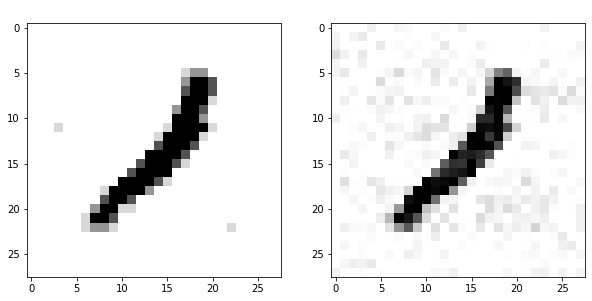
\includegraphics[width=7cm]{image_pertub_q5_n10_final.png}
	\caption{Image of 1 changed to 4 with the adversarial perturbation generated by the Decentralized Variance-Reduced Algorithm \ref{variance-reduced} with q=5 and n=10.}
	\label{fig:variance-reduced}
\end{figure}
In Figure \ref{fig:variance-reduced} we can see an example of the perturbations.
